\documentclass{standalone}

\usepackage[latin1]{inputenc}
\usepackage{amsmath}
\usepackage{amssymb}
\usepackage{amsthm}

\usepackage{tikz}
\usetikzlibrary{arrows,calc}

%% generates a tightly fitting border around the work
%\usepackage[active,tightpage]{preview}
%\PreviewEnvironment{tikzpicture}
%\setlength\PreviewBorder{0.5mm}
%%\renewcommand\PreviewBbAdjust{-\PreviewBorder 1mm -1.15mm -0.85mm}

\usepackage{color}

%\pagestyle{empty}

\begin{document}

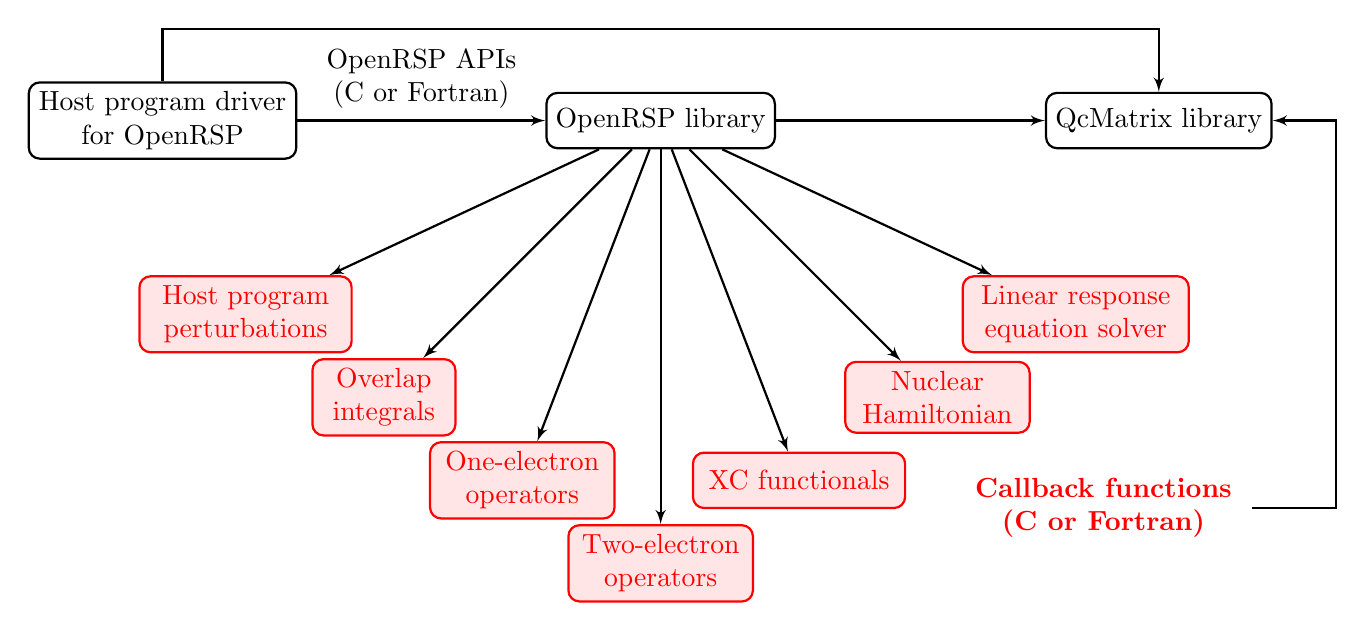
\begin{tikzpicture}[thick]
  \node[color=black, rectangle, draw, text badly centered, rounded corners, %
        minimum height=20] (OpenRSP) {OpenRSP library};
%
  \node[color=black, rectangle, draw, text badly centered, rounded corners, %
        minimum height=20, text width=90, left of=OpenRSP, node distance=180] %
       (HostDriver) {Host program driver for OpenRSP};
%
  \node[color=red, fill=red!10, rectangle, draw, text badly centered, rounded corners, %
        minimum height=20, text width=70, below of=OpenRSP, node distance=70, %
        xshift=-150, yshift=0] (Perturbations) {Host program perturbations};
  \node[color=red, fill=red!10, rectangle, draw, text badly centered, rounded corners, %
        minimum height=20, text width=45, below of=OpenRSP, node distance=70, %
        xshift=-100, yshift=-30] (Overlap) {Overlap integrals};
  \node[color=red, fill=red!10, rectangle, draw, text badly centered, rounded corners, %
        minimum height=20, text width=60, below of=OpenRSP, node distance=70, %
        xshift=-50, yshift=-60] (OneOper) {One-electron operators};
  \node[color=red, fill=red!10, rectangle, draw, text badly centered, rounded corners, %
        minimum height=20, text width=60, below of=OpenRSP, node distance=70, %
        xshift=0, yshift=-90] (TwoOper) {Two-electron operators};
  \node[color=red, fill=red!10, rectangle, draw, text badly centered, rounded corners, %
        minimum height=20, text width=70, below of=OpenRSP, node distance=70, %
        xshift=50, yshift=-60] (XCFun) {XC functionals};
  \node[color=red, fill=red!10, rectangle, draw, text badly centered, rounded corners, %
        minimum height=20, text width=60, below of=OpenRSP, node distance=70, %
        xshift=100, yshift=-30] (NucHamiltonian) {Nuclear Hamiltonian};
  \node[color=red, fill=red!10, rectangle, draw, text badly centered, rounded corners, %
        minimum height=20, text width=75, below of=OpenRSP, node distance=70, %
        xshift=150, yshift=0] (Solver) {Linear response equation solver};
  \node[color=red, text badly centered, minimum height=20, text width=100, %
        below of=Solver, node distance=70, xshift=10] (Callback) %
       {\textbf{Callback functions (C or Fortran)}};
%
  \node[color=black, rectangle, draw, text badly centered, rounded corners, %
        minimum height=20, right of=OpenRSP, node distance=180] %
       (QcMatrix) {QcMatrix library};
%
  \draw [-latex'] (HostDriver) edge node[align=center, midway, yshift=15, text width=120] %
    {OpenRSP APIs (C or Fortran)} (OpenRSP);
  \draw [-latex'] (OpenRSP)--(Perturbations);
  \draw [-latex'] (OpenRSP)--(Overlap);
  \draw [-latex'] (OpenRSP)--(OneOper);
  \draw [-latex'] (OpenRSP)--(TwoOper);
  \draw [-latex'] (OpenRSP)--(XCFun);
  \draw [-latex'] (OpenRSP)--(NucHamiltonian);
  \draw [-latex'] (OpenRSP)--(Solver);
  \draw [-latex'] (OpenRSP)--(QcMatrix);
  \draw [-latex'] (HostDriver.north) |- ($(QcMatrix.north)+(0,0.8)$) -- (QcMatrix);
  \draw [-latex'] (Callback.east) -| ($(QcMatrix.east)+(0.8,0)$) -- (QcMatrix);
\end{tikzpicture}

\end{document}
